% Chapter 3

\chapter{Corpus Models for Information Retrieval} % Main chapter title

\label{ir} % For referencing the chapter elsewhere, use \ref{Chapter3} 

\lhead{Chapter 3. \emph{Corpus Models for Information Retrieval}} % This is for the header on each page - perhaps a shortened title

%----------------------------------------------------------------------------------------

In this chapter, we will explain information retrieval briefly. After that we will the various corpus models used for
\textit{IR}. The popular \textit{LDA} model will be explained in detail later followed by it's evaluation. Let us first
see what is information retrieval.

\section{Information Retrieval}

\par 
In simple terms Information Retrieval is the process of retrieving information relevant to the need. As the web contains lot of
information, finding most relevant information is very difficult. A user usually requests information in the form of a query.
The retrieval engine then presents the user set of documents relevant to the user's query. As the web contains lot of noise, it
is difficult to fetch all the relevant documents. It should be noted that IR is not only concerned with the web as a resource of
information. Precision, Recall, and F-measure are the important performance measures of an IR system. They are defined as follows.

\subsection*{Precision}

\textit{Precision} is the fraction of documents that are relevant to the query

\begin{equation}
 Precision = \frac{|\{\textit{relevant documents}\} \cap \{\textit{retrieved documents}\}|}{|\{\textit{retrieved documents}\}|}
\end{equation}

\subsection*{Recall}

\textit{Recall} is the fraction of the documents that are relevant to the query that are successfully retrieved

\begin{equation}
 Recall = \frac{|\{\textit{relevant documents}\} \cap \{\textit{retrieved documents}\}|}{|\{\textit{relevant documents}\}|}
\end{equation}

\subsection*{F-measure}

\textit{F-measure} is the harmonic mean of \textit{Precision} and \textit{Recall}

\begin{equation}
 F = \frac{2.Precision.Recall}{(Precision+Recall)}
\end{equation}

\par

Text indexing, relevance ranking, similarity search and corpus modeling are amongst the most important approaches used for 
\textit{IR}. In the next section, we will show how sentiment analysis for sentiment-aware IR.

\section{Sentiment Aware IR}

In this section we will be discussing about two systems implemented to use \textit{sentiment analysis} in \textit{information retrieval}.

\begin{enumerate}
 \item Indexing followed by Sentiment Analysis
 \item Encoding sentiment in the Index
\end{enumerate}

As can be seen by the brief description, the first one uses a staged approach and the second one is a one-stage process but involves
some heavy preprocessing to predict the sentiment of the \textit{text}. These approaches are very simple and aren't novel.
These systems have merely been discussed to show the novelty of some future work. \textit{Lucene} \citep*{apachelucene} was used for indexing
in both these systems.

\subsection{Indexing followed by Sentiment Analysis}

\subsection*{Architecture}

\begin{enumerate}
 \item Lucene
  \par It has a variety of features to perform indexing from basic to very advanced. 
 \item Query Processor
  \par This is also a part of of lucene. The objective content of the query is processed by this component
 \item Sentiment Analyzer
  \par Sentiwordnet \citep*{sentiwordnet} was used to calculate the score of each word. The sentiment for a sentence was a sum of sentiment scores
  for each word. Sentiment of the whole document was a sum of sentiments for all the sentences. 
\end{enumerate}

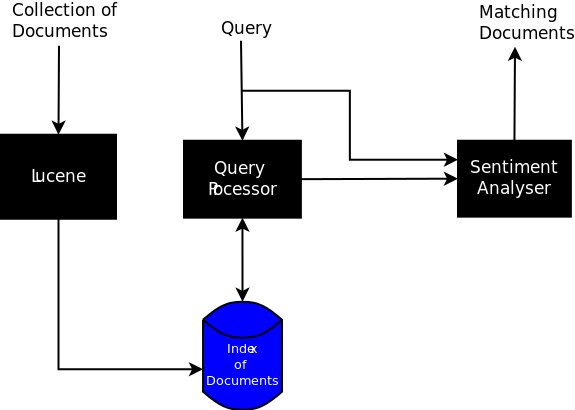
\includegraphics[width=\textwidth]{IndexingFollowedBySentimentAnalysis}
\begin{center}
 Figure 3.1 Indexing Followed by Sentiment Analysis
\end{center}

\subsection{Encoding sentiment in the Index}

\subsection*{Architecture}

\begin{enumerate}
 \item Lucene + Sentiment Analyzer
  \par It has a variety of features to perform indexing from basic to very advanced. In this case, sentiment analysis was combined with
  indexing. One more field, \textit{sentiment} was added to the index. This value was inferred using the sentiment analyzer. 
 \item Query Processor
  \par In this case, both the subjective and objective content of the query was processed. The documents were fetched based on the objective
  content of the query. Then, depending on the value of the \textit{sentiment} field, these fetched documents were filtered and presented
  to the user.
\end{enumerate}

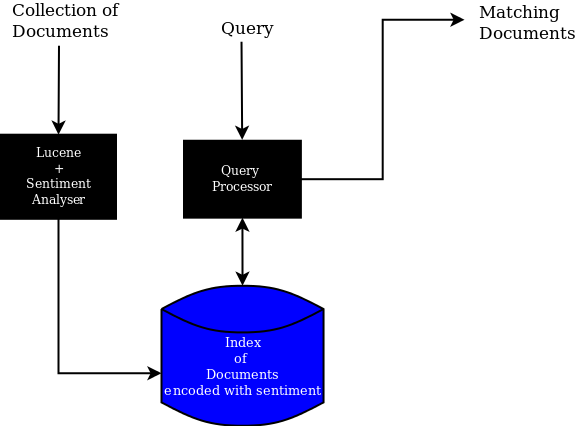
\includegraphics[width=\textwidth]{SentimentEncodedInIndex}
\begin{center}
 Figure 3.2 Encoding Sentiment in Index
\end{center}

Both these systems can be very useful. But as we can see the first one incurs lot of processing overhead and the second one has lot of 
preprocessing overhead. Also, both follow a procedural approach. A more novel approach will be two combine sentiment and topic to create 
a model which we can fit to our training data and then infer the resemblance of a new document to existing ones.

In this chapter we will focus on corpus modeling as in most works combining \textit{SA} and \textit{IR}, corpus modeling has been used. 
This draws directly from the Language Modeling approach used in many \textit{NLP} systems. In the next section we focus on the different
types of Corpus models. One effort towards using language modeling for \textit{IR} was made in \citep*{ponte1998language}

\section{Corpus Models}

Corpus models are the probabilistic language models using which we can perform retrieval. In this section, we will have a look 
at multivariate binary model, \textit{poisson} model, \textit{multinomial} model, \textit{DCM}, \textit{dirichlet} smoothed models, and \textit{LDA}. 
One advantage of using models to perform text retrieval is that the models can be refined independent of the retrieval algorithm. 

\subsection{Multivariate Binary Model}

A document in this model is represented as a bit vector where the presence or absence of a word in the vocabulary is represented 
by a bit. The probability of a document \(x\) is given by,

\begin{align}\label{eqn:multivariatebinary}
Pr(x \mid \phi )	& = \prod_{w \in W} {\phi_w}^{x_w}{(1-\phi_w)}^{1-x_w}\\
			& = \prod_{w \in W} \phi_w \prod_{w \in W, w \notin x} (1-\phi_w)
\end{align}

\(w\) in equation \ref{eqn:multivariatebinary} is a word in vocabulary \(W\). This model does not work well for short documents
because in that case \(|W| \gg |x|\). Also, the product  make strong independence assumptions leading to the underestimation of
\(Pr(x \mid \phi)\).

\subsection{Poisson Model}

In the previous model, word counts were not taken into consideration. For this model, the document will be represented by a
vector of word counts. Every word \(w\) has a parameter \(\mu_w\) associated with it. In this model, it is assumed that word
counts are random variables \(X_w\) that follow \textit{poisson} distributions with means \(\mu_w\) as follows:

\begin{equation}
 Pr(\textit{X_w = z}) = \frac{e^{-\mu_w}{\mu_w}^z}{z!}, \textit{z = 0,1,2,\dots}
\end{equation}

The probability of invoking the Poisson document generator and getting a count vector x is given as:

\begin{align}
 Pr(x \mid \mu)		& = \prod_{\textit{all w}} Pr(\textit{X_w = x_w}) \\
			& = \prod_{\textit{all w}} \frac{e^{-\mu_w}{\mu_w}^{x_w}}{x_w!} \\
			& = \textit exp(-\sum_{all w} \mu_w) \prod_{w \in x} \frac{{\mu_w}^{x_w}}{x_w!}
\end{align}

\subsection{Multinomial Model}

In the previous two models, we were not able to model the document length. In this model, we can take that aspect of the document
into consideration. Let \(L\) be the random variable for the document length. The length of the document in sampled from the 
distribution of this variable. For each word \(w\) in the vocabulary \(W\), a probability \(\theta_w\) is present. Let \(x_w\)
denote the count of word \(w\) and \(l_x\) denotes length of the document. 

The probability of the document with length \(l_x\) is given by:

\begin{align}
 Pr(l_x,\{ x_w \})	& = Pr(L=l_x)Pr(\{x_w\}|l_x,\theta) \\
			& = Pr(L=l_x) {{l_x} \choose {\{x_w\}}} \prod_{w \in x} {\theta_x}^{x_w} \\
			& = Pr(L=l_x) l_x! \prod_{w \in x} \frac{(\theta_x^{x_w}}{x_w!}
\end{align}

The drawback with the models discussed so far is that do not handle unknown words. If the document contains a word \(w\) which
is not in the vocabulary \(W\) then it's probability will be zero. The models we see next overcome this drawback. They also
take into account the word \textit{burstiness} which means that when a word appears once in a document, it tends to appear more. 

\subsection{Dirichlet distribution model}

In this model too the document is represented as a vector of word counts. The problem with multinomial model is that it fails to 
account for word \textit{burstiness}. The nature of data according to \textit{Zipf's} law follows a model of the form \({data}^{parameter}\) but in
case of multinomial it is \({parameter}^{data}\). It is this intuition that lead to look for new models for representing data.

Dirichlet distribution is a probability density function over distributions given as

\begin{equation}\label{eqn:dirichlet}
 p(\theta \mid \alpha) = \frac{\Gamma \Big( \sum_{w=1}^W \alpha_w \Big)}{\prod_{w=1}^W \Gamma (\alpha_w)} \prod_{w=1}^W {\theta_w}^{\alpha_w - 1}
\end{equation}

Equation \ref{eqn:dirichlet} can be written exponential family form as

\begin{equation}
 logp(\theta \mid \alpha) = \sum_{w=1}^W (\alpha_w - 1) log \theta_w + log \Gamma (\sum_{w=1}^W \alpha_w) - \sum_{w=1}^W log\Gamma(\alpha_w)
\end{equation}

In this model, the representation of the document is in terms of a probability vector. 

Documents being sparse in nature \textit{i.e}, each document contains only a small subset of the vocabulary which might make the probability
zero. Smoothing can be used in this case. 

\subsection{DCM (Dirichlet Compound Multinomial Model)}

The problem with using smoothing in \textit{DCM} is that over-smoothing is done. In this case all the rare words have the same probability
of appearing in all the classes. Since, rare words are the main discriminators in classification, this model is not suitable for
classification \citep*{madsen2005modeling}. A hierarchical model can solve this problem. \textit{DCM} is one such model. It was introduced in \citep*{madsen2005modeling}.

To generate a document using the \textit{DCM}, a sample is first drawn from the Dirichlet to get a multinomial distribution, then words are
iteratively drawn for the document based on the multinomial distribution. \textit{DCM} can be thought of as a bag-of-bag-of-words-model.
\citep*{madsen2005modeling}


The probability of a document \(x\) is given by:

\begin{equation}
 p(x \mid \alpha) = \int_\theta p(x \mid \theta ) p(\theta \mid \alpha) \mathrm{d}x 
\end{equation}

\subsection{Latent Dirichlet Allocation}

All the models discussed previously were for a single topic. We now consider one multi-topic model, \textit{LDA}. It was introduced in 
\citep*{blei2003latent}. Latent Dirichlet allocation is a way of automatically discovering topics that documents contain. 

In more detail, \textit{LDA} represents documents as mixtures of topics that spit out words with certain probabilities. It assumes that 
documents are produced in the following fashion: 

\begin{itemize}

\item When writing each document, you decide on the number of words N the document will have.

\item Choose a topic mixture for the document using dirichlet hypergenerator.

\item Generate each word in the document by:
  
  \begin{enumerate}
  
  \item First picking a topic using the multinomial distribution generated from the dirichlet hypergenerator.
  
  \item Then using the topic to generate the word itself.

  \end{enumerate}

\end{itemize}

Assuming this generative model for a collection of documents, LDA then tries to backtrack from the documents to find a set of 
topics that are likely to have generated the collection. A detailed discussion of LDA can be found in the next section.

\section{Latent Dirichlet Allocation}

\par

\textit{Latent Dirichlet Allocation} is a probabilistic generative model. It is completely unsupervised in nature. The main goal of 
\textit{LDA} is to do \textit{Latent Semantic Analysis} (\textit{LSA}). \textit{LSA} aims to find the latent structure of topics or 
concepts within a \textit{text}. \citep*{heinrich2005parameter} gives a very thorough explanation for \textit{LDA} and the inference 
method used. Most of the content in this chapter has been borrowed from \citep*{heinrich2005parameter}.

\subsection{Bayesian Network for LDA}

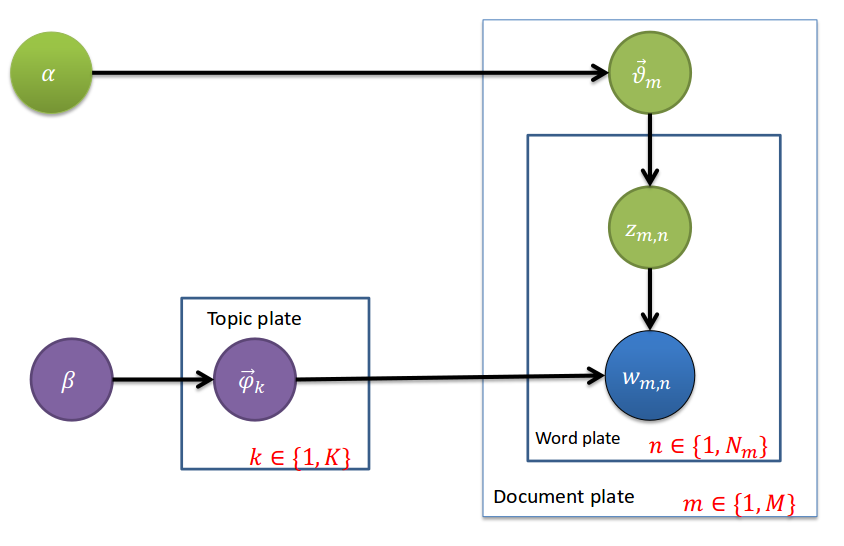
\includegraphics[width=\textwidth]{lda/lda.png} 
\begin{center}
 Figure 3.3 Bayesian Network for Latent Dirichlet Allocation
\end{center}

\textit{Bayesian Network} is a \textit{directed acyclic graph} (\textit{DAG}) where nodes correspond to random variables and edges correspond
to conditional probability distributions. The replication of a node is represented by a \textit{plate}. This is to account for multiple
values or mixture components.

\subsection{Generative Model for LDA}

The generative process for \textit{LDA} is as follows \(\colon\)

\begin{alltt}
\(\Box\) Topic Plate \(\colon\)
\textbf{for} all topics \( k \in [1,K] \) \textbf{do}
  sample mixture components \( \vec{\psi_k} \sim Dir(\vec{\beta}) \)
\textbf{end for}
\(\Box\) Document Plate \(\colon\)
\textbf{for} all documents \( m \in [1,M] \) \textbf{do}
  sample mixture proportion \( \vec{\vartheta_m} \sim Dir(\vec{\alpha}) \)
  sample document length \( N_m \sim Poiss(\xi)\)
  \(\Box\) Word Plate \(\colon\)
  \textbf{for} all words \( n \in [1,N_m] \) in document m \textbf{do}
    sample topic index \( z_{m,n} \sim Mult(\vec{\vartheta}_m) \)
    sample term for word \( w_{m,n} \sim Mult(\vec{\psi}_{z_{m,n}}) \)
  \textbf{end for}
\textbf{end for}
\end{alltt}

\subsection{Likelihoods}

Probability that a particular word \(w_{m,n}\) instantiates a particular term \(t\) given the \textit{LDA} parameters is,

\begin{equation}\label{eqn:likelihood}
 p(w_{m,n}=t|\vec{\vartheta}_m,\underline{\phi}) = \sum_{k=1}^{K} p(w_{m,n}=t|\vec{\psi}_k)p(z_{m,n}=k|\vec{\vartheta}_m)
\end{equation}

\eref{eqn:likelihood} corresponds to one iteration on the word plate of the bayesian network.

Joint distribution of all known and hidden variables given the hyperparameters is given by,

\begin{equation}
p(\vec{w}_m,\vec{z}_m,\vec{\vartheta}_m,\underline{\phi}|\vec{\alpha},\vec{\beta}) = 
\prod_{n=1}^{N_m} p(w_{m,n}|\vec{\psi}_{z_{m,n}})p(z_{m,n}|\vec{\vartheta}_m).p(\vec{\vartheta}_m|\vec{\alpha}).p(\underline{\phi}|\vec{\beta})
\end{equation}

Likelihood of one document is given by,

\begin{align}
p(\vec{w}_m|\vec{\alpha},\vec{\beta})		& = \iint p(\vec{\vartheta}_m|\vec{\alpha}).p(\underline{\phi}|\vec{\beta}).\prod_{n=1}^{N_m} \sum_{z_{m,n}} p(w_{m,n}|\vec{\psi}_{z_{m,n}})p(z_{m,n}|\vec{\vartheta}_m)d\underline{\phi}d\vec{\vartheta}_m \\                                  
						& = \iint p(\vec{\vartheta}_m|\vec{\alpha}).p(\underline{\phi}|\vec{\beta}).\prod_{n=1}^{N_m} p(w_{m,n}|\vec{\vartheta}_m,\underline{\phi}) d\underline{\phi}d\vec{\vartheta}_m
\end{align}

Likelihood of the whole corpus \(W = \{\vec{w}_m\}_{m=1}^{M}\) is given by,

\begin{equation}
p(W|\vec{\alpha},\vec{\beta}) = \prod_{m=1}^{M} p(\vec{w}_m|\vec{\alpha},\vec{\beta})
\end{equation}

Let us describe the quantities used in the model

\begin{alltt}
\(M\) number of documents to generate (const scalar).
\(K\) number of topics/mixture components (const scalar).
\(V\) number of terms \(t\) in vocabulary (const scalar).
\(\vec{\alpha}\) hyper-parameter on the mixing proportions (\(K-vector\) or scalar if symmetric).
\(\vec{\beta}\) hyper-parameter on the mixing components (\(K-vector\) or scalar if symmetric).
\(\vec{\vartheta}_m\) parameter notation for p(z|d=m), the topic mixture proportion for document \(m\). 
  One proportion for each document, \(\underline{\theta} = \{\vec{\vartheta}_m\} m=1 \cdots M (M \times K matrix)\).
\(\vec{\psi}_k\) parameter notation for p(t|z=k), the mixture component of topic \(k\). 
  One component for each topic, \(\underline{\phi} = \{\vec{\psi}_k\} k=1 \cdots K (K \times V matrix)\).
\(N_m\) document length (document-specific), here modeled with a Poisson distribution with 
  constant parameter \(xi\).
\(z_{m,n}\) mixture indicator that chooses the topic for the nth word in document m.
\(w_{m,n}\) term indicator for the nth word in document m.
\end{alltt}

\subsection{Inference via Gibbs Sampling}

The exact inference is intractable in case of \textit{LDA}. An approximate inference via \textit{Gibbs} sampling is used. 

\par
\textit{Gibbs} Sampling \citep*{walsh2004markov} is a special case of \textit{Markov-chain Monte Carlo}. \textit{MCMC} can emulate high dimensional probability
distributions, \(p(\vec{x})\) by the stationary distribution of a \textit{Markov chain}. Each sample is generated for each transition in 
the chain. This is done after a stationary state of the chain has been reached which happens after a so-called ``burn-in period'' which 
eliminates the effect of initialization parameters. In \textit{Gibbs} sampling, the dimensions \(x_i\) of the distribution are sampled
alternately one at a time, conditioned on the values of all other dimensions, denoted by \(\vec{x}_{ \neg i}\)

\subsubsection*{Bivariate Case of Gibbs Sampling}

\par
Consider a bivariate random variable \((x,y)\), and suppose we wish to compute the marginals, \(p(x)\) and \(p(y)\). The idea behind the
sampler is that it is easier to consider a sequence of distributions, \(p(x|y)\) and \(p(y|x)\) than obtaining the marginal by integration,
\(p(x) = \int p(x,y) dy\).

\textbf{Steps}

\begin{enumerate}
 \item Start with some initial value \(y_0\) for \(y\).
 \item Obtain \(x_0\) by generating a random variable from a conditional distribution, \(p(x|y=y_0)\).
 \item Use \(x_0\) to generate a new value of \(y_1\) drawing from a conditional distribution, \(p(y|x=x_0)\).
\end{enumerate}

The sampler proceeds as follows, 

\begin{enumerate}
 \item \(x_i \sim p(x|y=y_i)\)
 \item \(y_i \sim p(y|x=x_{i-1})\)
\end{enumerate}

Repeating this process \(k\) times generates a \textit{Gibbs} sequence of length \(k\), where a subset of points \((x_j,y_j)\) for 
\(1 \leq j \leq m < k\) are taken as simulated draws from the full joint distribution.

\subsubsection*{Multivariate Case}

The value of the \(k^{th}\) variable is drawn from the distribution, \(p(\theta^{(k)}|\Theta^{\neg k})\) where \(\Theta^{\neg k}\) denotes
a vector containing all the variables but \(k\). 

We draw from the distribution,

\(\theta_{i}^{(k)} \sim p(\theta^{(k)} | \theta^{(1)}=\theta_{i}^{(1)}, \cdots,\theta^{(k-1)}=\theta_{i}^{(k-1)},\theta^{(k+1)}=\theta_{i-1}^{(k+1)},\cdots,\theta^{(n)}=\theta_{i-1}^{(n)})\)

For example, if there are four variables, \((w,x,y,z)\), the sampler becomes

\begin{enumerate}
 \item \(w_i \sim p(w | x = x_{i-1}, y = y_{i-1}, z = z_{i-1})\)
 \item \(x_i \sim p(x | w = w_{i}, y = y_{i-1}, z = z_{i-1})\)
 \item \(y_i \sim p(y | w = w_{i}, x = x_{i}, z = z_{i-1})\)
 \item \(z_i \sim p(z | w = w_{i}, x = x_{i}, y = y_{i})\)
\end{enumerate}

\subsubsection*{Gibbs Sampling Algorithm}

To get a sample \(p(x)\),

\begin{enumerate}
 \item Choose dimension \(i\) (random or by permutation)
 \item Sample \(x_i\) from \(p(x_i|\vec{x}_{\neg i})\)
\end{enumerate}

\begin{equation}
 p(x_i|\vec{x}_{\neg i}) = \frac{p(\vec{x})}{p(\vec{x}_{\neg i})} where, \vec{x} = \{x_i,\vec{x}_{\neg i}\}
\end{equation}

\subsubsection*{Gibbs Sampling for Models with Hidden Variables}

For models containing hidden variable, \(\vec{z}\), their posterior given the evidence, \(p(\vec{z}|\vec{x})\) is a distribution commonly
wanted. 

The general formula of a \textit{Gibbs} sampler for such latent variable models becomes, 

\begin{equation}
 p(z_i|\vec{z}_{\neg i},\vec{x}) = \frac{p(\vec{z},\vec{x})}{p(\vec{z}_{\neg i},\vec{x})}
\end{equation}

\subsubsection*{LDA Gibbs Sampler}

Target of inference is the distribution, \(p(\vec{z}|\vec{w})\)

\begin{equation}
 p(\vec{z}|\vec{w}) = \frac{\vec{z},\vec{w}}{p(\vec{w})} = \frac{\prod_{i=1}^{W} p(z_i,w_i)}{\prod_{i=1}^{W} \sum_{k=1}^{K} p(z_i=k,w_i)}
\end{equation}

Full conditional, 

\begin{equation}\label{eqn:fullconditionalincomplete}
p(z_i|\vec{z}_{\neg i},\vec{w}) 
\end{equation}

is used to simulate \(p(\vec{z}|\vec{w})\)

This requires the joint distribution, 

\begin{equation}
p(\vec{w},\vec{z}|\vec{\alpha},\vec{\beta}) = p(\vec{w}|\vec{z},\vec{\beta})p(\vec{z}|\vec{\alpha})\label{eqn:wzgivenalphbetaincomplete}
\end{equation}

\subsubsection*{Calculation of \(p(\vec{w}|\vec{z},\vec{\beta})\)}

\(W\) words of the corpus are observed according to independent multinomial trials,

\begin{equation}
 p(\vec{w}|\vec{z},\underline{\phi}) = \prod_{i=1}^{W} p(w_i|z_i) = \prod_{i=1}^{W} \psi_{z_i,w_i}
\end{equation}

Splitting the product over words into product over topics and one over vocabulary,

\begin{equation}\label{eqn:wgivenpsi}
 p(\vec{w}|\vec{z},\underline{\phi}) = \prod_{k=1}^{K} \prod_{t=1}^{V} p(w_i=t|z_i=k) = \prod_{k=1}^{K} \prod_{t=1}^{V} \psi_{k,t}^{n_{k}^{t}}
\end{equation}

where, \(n_k^{(t)}\) denotes the number of times that the term \(t\) has been observed with topic \(k\).

Integrating \eref{eqn:wgivenpsi} over \(\underline{\phi}\) we get,

\begin{align}
  p(\vec{w}|\vec{z},\vec{\beta})	& = \int p(\vec{w}|\vec{z},\underline{\phi})p(\underline{\phi}|\vec{\beta})d\underline{\phi} \\
					& = \int \prod_{z=1}^{K} \frac{1}{\Delta(\vec{\beta})} \prod_{t=1}^{V} \psi_{z,t}^{n_{z}^{t}+\beta_t-1}d\vec{\phi}_z \\ 
					& = \prod_{z=1}^{K} \frac{\Delta(\vec{n}_z+\vec{\beta})}{\Delta(\vec{\beta})}, \vec{n}_z = \{n_{z}^{(t)}\}_{t=1 \cdots N}
					\label{eqn:wgivenbeta}
\end{align}

\subsubsection*{Calculation of \(p(\vec{z}|\vec{\alpha})\)}

\begin{align}
 p(\vec{z}|\underline{\theta})		& = \prod_{i=1}^{W} p(z_i|d_i) \\
					& = \prod_{m=1}^{M} \prod_{k=1}^{K} p(z_i=k|d_i=m) \\
					& = \prod_{m=1}^{M} \prod_{k=1}^{K} \vartheta_{m,k}^{n_m^{k}} \label{eqn:zgiventheta}
\end{align}

where, \(d_i\) refers to the document a word \(i\) belongs to and \(n_m^{(k)}\) refers to the number of times that topic \(k\) has been observed
with a word of document \(m\).

Integrating \eref{eqn:zgiventheta} over \(\underline{\theta}\) we get,

\begin{align}
 p(\vec{z}|\vec{\alpha})		& = \int p(\vec{z}|\underline{\theta})p(\underline{\theta}|\vec{\alpha})d\underline{\theta} \\
					& = \int \prod_{m=1}^{M} \frac{1}{\Delta(\vec{\alpha})} \prod_{k=1}^{K} \vartheta_{m,k}^{n_m^{k} + \alpha_k - 1} d\vec{\vartheta}_m \\
					& = \prod_{m=1}^{M} \frac{\Delta(\vec{n}_m+\vec{\alpha})}{\Delta(\vec{\alpha})}, \vec{n}_m = \{n_{m}^{(k)}\}_{k=1 \cdots K}
					\label{eqn:zgivenalpha}
\end{align}

Putting \eref{eqn:zgivenalpha} and \eref{eqn:wgivenbeta} into \eref{eqn:wzgivenalphbetaincomplete} we get,

\begin{equation}\label{eqn:jointdistribution}
p(\vec{z},\vec{w}|\vec{\alpha},\vec{\beta}) = \prod_{z=1}^{K} \frac{\Delta(\vec{n}_z+\vec{\beta})}{\Delta(\vec{\beta})} \prod_{m=1}^{M} \frac{\Delta(\vec{n}_m+\vec{\alpha})}{\Delta(\vec{\alpha})}
\end{equation}

\eref{eqn:jointdistribution} is the joint distribution. 

Now, the full conditional given in \eref{eqn:fullconditionalincomplete} can be expressed as,
 
\begin{align}
p(z_i=k|\vec{z}_{\neg i},\vec{w})	& = \frac{p(\vec{w},\vec{z})}{p(\vec{w},\vec{z}_{\neg i})} \\
					& = \frac{p(\vec{w}|\vec{z})p(\vec{z})}{p(\vec{w}|\vec{z}_{\neg i})p(\vec{z}_{\neg i})} \\
					& \propto \frac{\Delta(\vec{n}_z+\vec{\beta})}{\Delta(\vec{\beta})} . \frac{\Delta(\vec{n}_m+\vec{\alpha})}{\Delta(\vec{\alpha})} \\
					& \propto \frac{\Gamma(n_{k}^{(t)} + \beta_t)\Gamma(\sum_{t=1}^{V} n_{k,\neg i}^{(t)} + \beta_t)}{\Gamma(n_{k,\neg i}^{(t)} + \beta_t)\Gamma(\sum_{t=1}^{V} n_{k}^{(t)} + \beta_t)}.
						  \frac{\Gamma(n_{m}^{(k)} + \alpha_k)\Gamma(\sum_{k=1}^{K} n_{m,\neg i}^{(k)} + \beta_t)}{\Gamma(n_{m,\neg i}^{(k)} + \beta_t)\Gamma(\sum_{k=1}^{K} n_{m}^{(k)} + \beta_t)} \\
					& \propto \frac{n_{k,\neg i}^{(t)} + \beta_t}{\sum_{t=1}^{V}n_{k,\neg i}^{(t)} + \beta_t}.
						  \frac{n_{m,\neg i}^{(k)} + \alpha_k}{[\sum_{k=1}^{K}n_{m,\neg i}^{(k)} + \alpha_k]-1}
					\label{eqn:fullconditionalfinal}
\end{align}

where the counts \(n_{.,\neg i}^{(.)}\) indicate that the token \(i\) is excluded from the corresponding document or topic.

\subsubsection*{Multinomial parameters}

The multinomial parameter sets, \(\underline{\Theta}\) and \(\underline{\phi}\) that correspond to the state of the Markov
chain, \(M={\vec{w},\vec{z}}\) can be obtained as follows

\begin{equation}\label{eqn:multtheta}
p(\vec{\vartheta}_m|M,\vec{\alpha}) = \frac{1}{Z_{\vartheta_m}} \prod_{n=1}^{N_m} p(z_{m,n}|\vec{\vartheta}_m) p(\vec{\vartheta}_m|\vec{\alpha}) = 	Dir(\vec{\vartheta}_m|\vec{n}_m + \vec{\alpha})
\end{equation}

\begin{equation}\label{eqn:multphi}
p(\vec{\psi}_k|M,\vec{\beta}) = \frac{1}{Z_{\psi_k}} \prod_{k=1}^{K} p(w_{i}|\vec{\psi}_k) p(\vec{\psi}_k|\vec{\beta}) = 	Dir(\vec{\psi}_k|\vec{n}_k + \vec{\beta}) 
\end{equation}

Using the expectation of the dirichlet distribution, \(Dir(\vec{\alpha}) = \frac{a_i}{\sum_i a_i}\) in \eref{eqn:multtheta} and \eref{eqn:multphi} we get,

\begin{equation}\label{eqn:phi}
\psi_{k,t} = \frac{n_k^{(t)} + \beta_t}{\sum_{t=1}^{V} n_k^{(t)} + \beta_t}
\end{equation}

\begin{equation}\label{eqn:theta}
\vartheta_{m,k} = \frac{n_m^{(k)} + \alpha_t}{\sum_{k=1}^{K} n_m^{(k)} + \alpha_k} 
\end{equation}

\pagebreak

\subsection*{Gibbs Sampling Algorithm for LDA}

\begin{alltt}
\(\Box\) Initialization
zero all count variables, \(n_m^{(k)},n_m,n_k^{(t)},n_k\)
for all documents \(m \in [1,M]\) do
  for all words \(n \in [1,N_m]\) in document \(m\) do
    sample topic index \(z_{m,n} = k \sim Mult(1/K)\)
    increment document-topic count: \(n_m^{(k)} + 1\)
    increment document-topic sum: \(n_m + 1\)
    incremnet topic-term count: \(n_k^{(t)} + 1\)
    increment topic-term sum: \(n_k + 1\)
  end for
end for
\(\Box\) Gibbs sampling over burn-in period and sampling period
while not finished do
  for all documents \(m \in [1,M]\) do
    for all words \(n \in [1,N_m]\) in docuemnt \(m\) do
      \(\Box\) for the current assignment of \(k\) to a term \(t\) for word \(w_{m,n}\) \(\colon\)
      decrement counts and sum:\(n_m^{k}-1,n_m-1,n_k^{(t)}-1,n_k-1\)
      \(\Box\) multinomial sampling according to \eref{eqn:fullconditionalfinal} (decrements from the previous step)
      sample topic index \(\bar{k} \sim p(z_i|\vec{z}_{\neg i},\vec{w})\)
      \(\Box\) use the new assignment of \(z_{m,n}\) to the term \(t\) for word \(w_{m,n}\) to:
      increment the counts and sum:\(n_m^{k}+1,n_m+1,n_k^{(t)}+1,n_k+1\)
    end for
  end for
  \(\Box\) check convergence and read out parameters
  if converged ad \(L\) sampling iterations since last read out then
    \(\Box\) the different parameters read outs are averaged
    read out parameter set \(\underline{\phi}\) according to \eref{eqn:phi}
    read out parameter set \(\underline{\theta}\) according to \eref{eqn:theta}
  end if
end while
\end{alltt}

\subsection{Inferencing}

Inferencing is the process of finding out the topic distribution in a new document. Suppose the new document is represented by \(\bar{m}\),
Let us represent a new document by \(\vec{w}\). We need to find out the posterior distribution of topics \(\vec{z}\) given the word 
vector of the document \(\vec{w}\) and the \textit{LDA Markov} state, \(M = \{ \vec{z},\vec{w} \} \colon p(\vec{z},\vec{w};M) \).

The algorithm is a modification the \textit{Gibbs} sampling algorithm we saw. It starts of by randomly assigning topics to words and then
performs number of loops through the \textit{Gibbs} sampling update (locally for the words \(i\) of \(\bar{m}\)) \citep*{heinrich2005parameter}.

\begin{equation}\label{eqn:inferencereqn}
p(\bar{z}_i=k | \bar{w}_i=t,\bar{\vec{z}}_{\neg i},\bar{\vec{w}}_{\neg i};M) =
\frac{n_{k}^{(t)} + \bar{n}_{k,\neg i}^{(t)} + \beta_t}{\sum_{t=1}^{V} n_{k}^{(t)} + \bar{n}_{k,\neg i}^{(t)} + \beta_t}.
\frac{n_{\bar{m},\neg i}^{(k)} + \alpha_k}{[\sum_{k=1}^{K} n_{\bar{m},\neg i}^{(k)} + \alpha_k]-1}
\end{equation}

where \(\bar{n}_{k}^{t}\) counts the observations of term \(t\) and topic \(k\) in the new document.

The topic distribution of the new document can be found out using the following equation,

\begin{equation}
\vartheta_{\bar{m},k} = \frac{n_{\bar{m}}^{(k)} + \alpha_k}{\sum_{k=1}^{K} n_{\bar{m}}^{(k)} + \alpha_k} 
\end{equation}

In the next section, we will evaluate \textit{LDA}.

\section{Evaluation of LDA}

Evaluation of topic models has been discussed at length in \citep*{wallach2009evaluation}. A natural evaluation metric discussed in 
\citep*{wallach2009evaluation} is finding out the probability of a held-out document given a trained model. Topic modeling is a useful
tool for analyzing unstructured text collections. Evaluation of topic models is difficult due to their unsupervised nature. For some 
applications, there might be extrinsic tasks such as information retrieval for which performance can be evaluated. There is a need for 
a universal method that measures generalization capability of a topic model in a way that is accurate, computationally efficient and
independent of a specific application. \textit{LDA} can be evaluated by 1) Information retrieval accuracy or 2) by estimating the probability
of unseen held-out documents given some training documents. We propose a new evaluation method as follows.

\subsection*{Evaluation method}

\begin{enumerate}
 \item Download documents.
 \item Tag every document with a topic to get a tagged corpus
 \item Held-out some documents for testing before training the model
 \item Train the topic model usingd the untagged corpus (obtained after removing the tags)
 \item Now, use the trained model to infer topic distribution for the testing documents
 \item Check whether the topic having highest proportion matches the tag of the document
\end{enumerate}

5-fold cross validation was used in this case. 1273 documents were downloaded from DMOZ \citep*{dmoz}. Computers, films, real estate, cooking and
sports were the 5 topics chosen. The implementation in Mallet was used to conduct the experiment.

\begin{center}
\begin{tabular}{ |c|c| }
  \hline
  Topic & No. of files \\ \hline
  Computers & 164 \\ \hline
  Sports & 213 \\ \hline
  Cooking & 251 \\ \hline
  Real Estate & 261 \\ \hline
  Films & 384 \\ \hline
\end{tabular}
\end{center}
\begin{center}
 Table 3.1 Number of files per topic
\end{center}

\begin{center}
\begin{tabular}{ |c|c| }
  \hline
  Average accuracy & 20.867 \\ \hline
\end{tabular}
\end{center}
\begin{center}
 Table 3.2 Average Accuracy 
\end{center}

\subsection*{Discussion}

\par
The average accuracy after 5-fold cross-validation on this corpus was 20.867, which is very low. The reason for this is the short-length
of the documents used. \textit{LDA} works on the principle of co-occurrence. If we look at \eref{eqn:fullconditionalfinal}, there is a
factor for words and another for documents. Probabilities are higher for assignments that "don't break document boundaries", that is, words 
appearing in the same document have a slightly higher odds of ending up in the same topic. The same holds for document assignments, they to 
a degree follow "word boundaries". These effects mix up and spread over clusters of documents and words, eventually. Due to the short length 
of the documents, words from the same topic may not always co-occur. Also, there is chance of them co-occurring with words from other topics 
also which results in bad clustering. Some words belong to more than one topic due to this. Due to this, the clustering of documents as whole 
in this case is not good. 

\par
Also, the evaluation method used is very strict. If it is a bit lenient, the accuracy can be increased. A new method
called weighted evaluation can be used in this case.

\subsection*{Weighted Evaluation}

Weighted evaluation is based on the fact that we get a topic distribution for each testing document. This topic distribution is arranged
in descending order of topic proportions. The idea is to assign weights according to the rank given to the original tag of the document. 

\subsection*{Weighted Evaluation Algorithm}

\begin{alltt}
matches=0, counts=0
For each document
  Find topic distribution
  Switch(tag):
    case(topic1): matches += 1
    case(topic2): matches += 0.8
    case(topic3): matches += 0.6
    case(topic4): matches += 0.4
    case(topic5): matches += 0.2
    counts++
Accuracy = matches/counts
\end{alltt}

\subsection*{Results}

\begin{center}
\begin{tabular}{ |c|c|c|c| }
  \hline
  Fold & Matches & Counts & Accuracy (in percentage) \\ \hline
  Fold 1 & 156 & 255 & 61.4 \\ \hline
  Fold 2 & 156 & 255 & 61.4 \\ \hline
  Fold 3 & 170 & 255 & 66.9 \\ \hline
  Fold 4 & 152 & 255 & 59.6 \\ \hline
  Fold 5 & 161 & 253 & 63.9 \\ \hline
\end{tabular}
\end{center}
\begin{center}
 Table 3.3 Accuracy for each testing fold 
\end{center}

\begin{center}
\begin{tabular}{ |c|c| }
  \hline
  Average accuracy & 62.6 \\ \hline
\end{tabular}
\end{center}
\begin{center}
 Table 3.4 Weighted Evaluation Average Accuracy 
\end{center}

\subsection*{Discussion}

\par
As we can see the accuracy has increased after we used weighted evaluation. This kind of evaluation needs to be used in many systems including
transliteration where the most probable word needs to be predicted. The rank of the actual word may be further down. This doesn't mean that the
system is giving wrong output. Therefore, a more lenient approach would be better in this case. 

\par
The accuracy has increased but still is unsatisfactory. 62 \% accuracy in this case implies that given a document, there is 62 \%
chance that the main topic of the document will be ranked in top 5. As we have used only 5 topics, this result is not that significant. Using
more number of topics will lead to better insights. 

\par 
If we consider the clustering to be effective only till the third rank, we get accuracies as shown in the table.

\begin{center}
\begin{tabular}{ |c|c|c|c| }
  \hline
  Fold & Matches & Counts & Accuracy (in percentage) \\ \hline
  Fold 1 & 156 & 255 & 50.9 \\ \hline
  Fold 2 & 156 & 255 & 50.1 \\ \hline
  Fold 3 & 170 & 255 & 57.4 \\ \hline
  Fold 4 & 152 & 255 & 46.7 \\ \hline
  Fold 5 & 161 & 253 & 53.5 \\ \hline
\end{tabular}
\end{center}
\begin{center}
 Table 3.5 Accuracy for each testing fold (Till 3rd rank)
\end{center}

\begin{center}
\begin{tabular}{ |c|c| }
  \hline
  Average accuracy & 51.7 \\ \hline
\end{tabular}
\end{center}
\begin{center}
 Table 3.6 Average Accuracy (Till 3rd rank)
\end{center}

\par 

This means that given a document, there is 51.7 \% chance that the main topic of the document will be ranked in top 3. It is known
that \textit{LDA} performs better with more number of topics. So, increasing the number of topics while performing the evaluation can 
lead to more better results. 

A list of high probability words for each topic was prepared which is given in the following table. 

\begin{center}
\begin{tabular}{ |c|c|c|c|c| }
  \hline \hline
  Computer & Films & Cooking & Real Estate & Sports \\ \hline \hline
  site & film &	recipes & services & reviews \\ \hline
  software & information & recipe & real & news \\ \hline
  free & offers & including & company &	interviews\\ \hline
  systems & production & collection & estate & information \\ \hline
  programming & courses & tips & includes & features \\ \hline
  research & links & source & commercial & current \\ \hline
  resources & videos & production & based & tennis \\ \hline
  code & television & baking & development & running \\ \hline
  information &	cinema & breakfast & title & tournament \\ \hline
\end{tabular}
\end{center}
\begin{center}
 Table 3.7 High probability words in each topic 
\end{center}

As we can see, the high probability words in each topic are good but due to the short length, results were not that good. 

\section*{SUMMARY}

We started with an introduction of \textit{IR}. Popular approaches for IR were listed. We had a detailed discussion on corpus models like
multivariate binary model, poisson model, multinomial model, dirichlet smoothed model, \textit{DCM} and \textit{LDA}. The generative modeling 
it uses, inference procedure and evaluation. 

The main goal of this project is to make use of generative models for sentiment analysis. In the next chapter we focus on some existing work 
in this direction. We also show how can \textit{LDA} and topical n-grams model be used for sentiment analysis.

\clearpage
